\documentclass[conference]{IEEEtran}
\IEEEoverridecommandlockouts
\usepackage{cite}
\usepackage{amsmath,amssymb,amsfonts}
\usepackage{graphicx}
\usepackage{textcomp}
\usepackage{xcolor}
\usepackage{array}
\usepackage{booktabs}
\usepackage{multirow}
\usepackage{url}
\graphicspath{{figures/}{./}}

\begin{document}

\title{An Agentic AI and IoT-Based Intelligent Soil Monitoring and Precision Irrigation Management System for Mango Orchards}

\author{\IEEEauthorblockN{Jayprakash}
\IEEEauthorblockA{\textit{Dept. of Electronics and Communication Engineering, Pranveer Singh Institute of Technology}, Kanpur, Uttar Pradesh, India\\

jpbjayprakash@gmail.com}
}

\maketitle

\begin{abstract}
Mango orchards need a growth-stage-dependent water regime: a planned dry spell before flowering, adequate moisture from flowering to fruit maturity, and reduced irrigation before harvest. This paper presents an agentic irrigation system that combines ESP32 soil-moisture nodes, an MQTT/HTTP backend, a Double Deep Q-Network (DQN) planner and a deterministic safety guard that has the final word on the valve. A single-layer root-zone water balance driven by Hargreaves reference evapotranspiration and a stochastic weather generator calibrated to India Meteorological Department (IMD) normals for Lucknow is used for training and evaluation. Over 30 unseen weather years (958$\pm$284~mm rain), the agentic policy kept the root zone inside the stage-specific target band on 72.2\% of days, against 63.4\% for a threshold rule, 9.6\% for a fixed calendar schedule and 33.9\% without irrigation. Days below the band fell from 9.8\% to 1.0\% ($p<10^{-5}$, Wilcoxon signed-rank) for only 7~mm (0.9\%) more water per year, while the calendar schedule applied 1464~mm and lost 1035~mm to deep drainage. In a sensor-fault stress test, the guard prevented 1200~mm of erroneous irrigation caused by a dead probe and raised an alert on every faulty day, whereas the DQN alone flooded the root zone. All results are simulation-based and conditional on assumed soil and crop parameters; Section~\ref{sec:limits} sets out the field validation that is still required.
\end{abstract}

\begin{IEEEkeywords}
Agentic AI, Internet of Things, deep reinforcement learning, Double DQN, precision irrigation, soil moisture, mango, ESP32, MQTT
\end{IEEEkeywords}

\section{Introduction}
\IEEEPARstart{A}{griculture} remains central to India's food security and rural employment, and mango is among its most important fruit crops, consumed in large volumes at home and exported when quality allows. Through most of the year a mango tree responds strongly to its environment. Soil moisture, air temperature and canopy humidity influence the timing of flowering, the success of fruit set, the rate of fruit growth and the risk of disease. Water is the most delicate of these factors, because more of it does not always help: growers commonly withhold water in the weeks before flowering, keep the soil moist from flowering until the fruit approaches maturity, and cut back again shortly before harvest~\cite{ntdaf,wfp}. An orchard manager therefore needs two pieces of knowledge together: how wet the soil is now, and how wet it ought to be at this point in the season.

Most growers still answer that question by inspecting the soil by hand and watering by habit or by the calendar. The approach is cheap, but it is labour-intensive, cannot run day and night, and leaves no record that can inform later decisions. Low-cost sensors and wireless communication offer an alternative: Internet-of-Things (IoT) irrigation systems place battery-powered nodes in the field, relay readings to the cloud and let the grower check conditions remotely~\cite{garcia2020,goap2018}. Many such installations, however, only display numbers or apply one fixed moisture threshold. They ignore the growth stage, cannot account for rain that is about to arrive, and cannot distinguish a dry field from a faulty sensor.

Reinforcement learning (RL) suits irrigation because the task is sequential, the weather is uncertain and the consequences of a decision appear days later. RL controllers have been trained for rice using weather forecasts~\cite{chen2021}, compared across on- and off-policy algorithms for tomato~\cite{alibabaei2022}, and deployed in an almond orchard with a safety fallback~\cite{ding2022}. A Deep Q-Network (DQN)~\cite{mnih2015} estimates the value of each discrete action with a neural network. A more recent idea is the \emph{agentic} pattern, in which software reasons, acts through tools and observes the outcome~\cite{yao2023}. In an orchard such an agent reads the sensors, considers the growth stage and the weather, proposes an irrigation depth, checks it against safety rules, operates the valve and explains the decision to the farmer. Because a learned policy should never hold unchecked authority over a valve, a rule-based guard is placed between the learner and the hardware.

This paper presents such a system for mango. Its contributions are:
\begin{enumerate}
\item A complete field-to-dashboard pipeline: ESP32 nodes sense the orchard, data travel over MQTT or HTTP to a FastAPI backend, and valve commands return to the field with a local fail-safe timer.
\item An agent that couples a Double-DQN irrigation planner with a deterministic safety guard that checks every proposal against rain, soil state, growth stage, a weekly water budget and sensor health.
\item A growth-stage-aware soil-water simulator for mango, driven by a stochastic weather generator calibrated to IMD climatological normals for Lucknow, the centre of Uttar Pradesh's mango belt.
\item A statistical comparison against three baselines on 30 unseen weather years, and a sensor-fault stress test that isolates the contribution of the guard; code, data and figures are released for reproduction.
\end{enumerate}

\section{Background and Related Work}

\subsection{Stage-Aware Irrigation in Mango}
\label{sec:bg-stage}
Advice from mango-growing regions follows a common outline. According to the Northern Territory guidelines, mature trees are kept dry between the close of the wet season and flowering, watering stops some weeks ahead of harvest, and growers are advised to track soil water with tensiometers, neutron probes or capacitance probes~\cite{ntdaf}. The Queensland \emph{Water for Profit} benchmark gives a similar sequence: begin watering once the majority of flower buds are developing, prevent stress through flowering and fruit set, ease off one to two weeks ahead of harvest, and resume as soon as the crop is picked~\cite{wfp}. In India, a four-year trial on the hybrid `Amrapali' compared drip irrigation at 25\%, 50\% and 75\% of pan-evaporation replenishment with and without mulch and reported the best growth, fruit retention and yield at 75\% replenishment~\cite{samant2017}. Stem-level studies under different irrigation regimes~\cite{hahn2022} and trials of regulated deficit and partial root-zone drying in `Chok Anan'~\cite{spreer2009} further show that the timing of water stress matters as much as its amount. For a controller, the implication is that the moisture target must change with the season.

\subsection{Sensing and Learning-Based Control}
Capacitive soil-moisture probes are inexpensive and easy to integrate into IoT nodes, but low-cost units vary from unit to unit and need soil-specific calibration~\cite{placidi2020}. IoT irrigation surveys report that most deployed systems still use fixed thresholds or simple rules~\cite{garcia2020}, while machine-learning variants mainly predict soil moisture rather than decide when to irrigate~\cite{goap2018}. On the decision side, DQN~\cite{mnih2015} and its Double-DQN refinement, which reduces over-estimation of action values~\cite{vanhasselt2016}, are widely used value-based methods. DRLIC~\cite{ding2022} is closest in spirit to this work: it pairs a deep-RL agent with a safety module that falls back to evapotranspiration-based control, and reported 9.52\% water savings in a 15-day field test on almond trees. Alibabaei \textit{et al.}~\cite{alibabaei2022} found that an on-policy A2C agent used about 20\% less water than DQN for tomato, and Chen \textit{et al.}~\cite{chen2021} used weather forecasts inside an RL irrigation policy for rice.

\subsection{Research Gap}
\begin{itemize}
\item Monitoring-only systems display data but neither decide nor explain.
\item Learned controllers are rarely evaluated against hardware faults, although a dead or frozen probe is a common failure in the field.
\item None of the systems above encodes the stage-dependent water regime of mango, including the planned dry spell before flowering.
\end{itemize}

\section{System Architecture}
Fig.~\ref{fig:arch} shows the system, organised in six layers (Table~\ref{tab:arch}).

\begin{figure*}[!t]
\centering
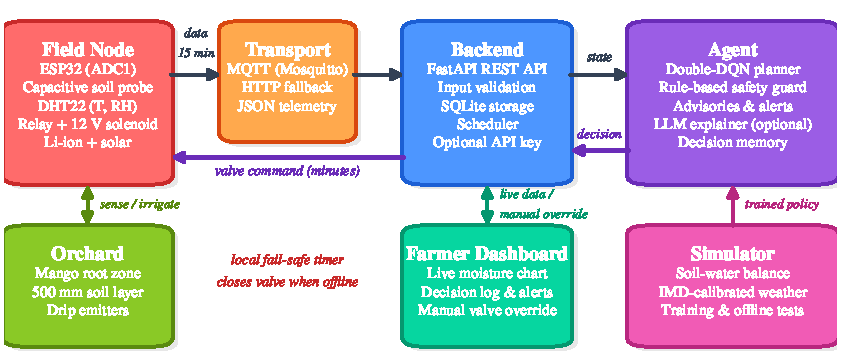
\includegraphics[width=0.92\textwidth]{fig1_architecture.pdf}
\caption{System architecture. ESP32 field nodes publish telemetry over MQTT/HTTP to a FastAPI backend; the agent returns an irrigation decision that is converted into valve minutes. The simulator supplies the trained policy, and the dashboard provides live data and manual override.}
\label{fig:arch}
\end{figure*}

\begin{table}[!t]
\caption{System Layers and Their Roles}
\label{tab:arch}
\centering
\footnotesize
\renewcommand{\arraystretch}{1.12}
\begin{tabular}{@{}>{\raggedright\arraybackslash}p{0.16\columnwidth}>{\raggedright\arraybackslash}p{0.35\columnwidth}>{\raggedright\arraybackslash}p{0.38\columnwidth}@{}}
\toprule
\textbf{Layer} & \textbf{Components} & \textbf{Role} \\
\midrule
Field node & ESP32, capacitive soil probe, DHT22, relay and solenoid valve & Reads every 15 min, publishes JSON, closes the valve on a local timer even when offline \\
Transport & MQTT (Mosquitto), HTTP & Telemetry in, valve commands out \\
Backend & FastAPI, SQLite & Validates input, stores data, schedules work, serves the REST API \\
Agent & Double-DQN planner, safety guard, advisories, optional LLM explainer & Perceive, reason, guard, act, remember \\
Interface & Web dashboard & Live chart, decision log, alerts, manual valve control \\
Simulator & Soil-water balance, weather generator & Training and offline testing \\
\bottomrule
\end{tabular}
\end{table}

\subsection{The Agent Loop}
The daily decision cycle is shown in Fig.~\ref{fig:loop}.
\begin{enumerate}
\item \textit{Perceive:} gather the 24-h median soil moisture, temperature and humidity, today's rain and tomorrow's forecast, the growth stage from the calendar and the days since the last irrigation.
\item \textit{Reason:} the DQN scores four actions (0, 6, 12 or 20~mm) and proposes the best.
\item \textit{Guard:} irrigation is blocked if more than 2~mm of rain falls or at least 8~mm is forecast, if the soil is above the band, or during the pre-flowering dry phase unless the soil is near wilting (below 14\% VWC). A single event is capped at 20~mm and a rolling seven-day budget of 60~mm applies. If the reading is absent, implausible ($<2\%$ or $>45\%$) or unchanged for three consecutive days, no water is released and an alert is raised. Outside pre-flowering, soil near wilting triggers an emergency 12~mm.
\item \textit{Act:} the depth is converted into valve minutes using the drip application rate and sent by MQTT or returned in the HTTP reply.
\item \textit{Remember and explain:} the decision, its reasons and a plain-language note are stored. An optional language model may rephrase the note but never changes the amount of water.
\end{enumerate}

\begin{figure}[!t]
\centering
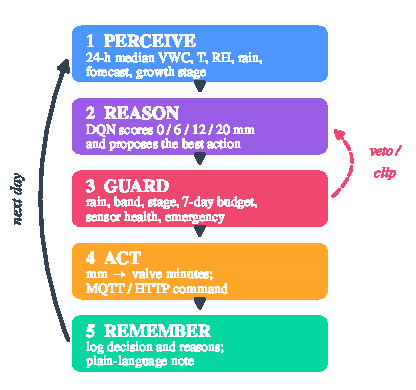
\includegraphics[width=0.86\columnwidth]{fig2_agent_loop.pdf}
\caption{Daily agent loop. The guard can veto or clip the planner's proposal before any valve command is issued.}
\label{fig:loop}
\end{figure}

\section{Methodology}

\subsection{Weather Generator}
Daily weather for Lucknow (26.9$^\circ$N) is generated stochastically from IMD climatological normals (temperature and rainfall 1971--2000, rainy days 1981--2010)~\cite{imd}. Rain occurrence follows a two-state Markov chain whose stationary wet-day probability equals the IMD rainy-day frequency of each month (persistence factor 0.4). Wet-day amounts are $2.5~\text{mm}+\text{Gamma}(k{=}0.8)$, scaled so the expected monthly total matches the normal, and each year receives a log-normal multiplier ($\sigma=0.25$) to reproduce inter-annual variability. Maximum and minimum temperatures follow the monthly normals with an AR(1) anomaly ($\sigma=1.5^\circ$C, $\phi=0.7$), and mean humidity is derived assuming dew point $\approx T_{\min}$~\cite{allen1998}. Over 200 generated years the mean annual rainfall is 966~mm against the IMD normal of 990~mm, and every monthly mean lies close to its normal (Fig.~\ref{fig:climate}a). The next-day rain forecast is the true value with log-normal noise ($\sigma=0.5$), 15\% missed events and 8\% false alarms.

\subsection{Soil-Water Model}
The root zone is a single 500~mm layer, so 1~mm of water changes volumetric water content (VWC) by 0.2 percentage points. The daily balance is
\begin{equation}
S_t = S_{t-1} + P_t + I_t - ET_{a,t} - D_t,
\end{equation}
where $S_t$ is stored water, $P_t$ rainfall, $I_t$ irrigation, $ET_{a,t}$ actual evapotranspiration and $D_t$ drainage. Reference evapotranspiration $ET_0$ is computed with the Hargreaves equation~\cite{hargreaves2003}, recommended by FAO-56 when radiation, wind and humidity data are unavailable~\cite{allen1998}, using extraterrestrial radiation for the site latitude. Then $ET_{a}=K_s K_c ET_0$, where $K_c$ is a stage-specific crop coefficient (assumed 0.70, 0.85, 1.00, 0.90 and 0.80 for the five stages) and $K_s$ is the FAO-56 water-stress coefficient with depletion fraction $p=0.5$. Half of any water above field capacity (32\% VWC) drains each day, water above saturation (42\%) is lost immediately, and the wilting point is 12\%.

\subsection{Target Bands}
Table~\ref{tab:bands} and Fig.~\ref{fig:climate}b list the stage-wise bands. They are default values chosen to follow the qualitative advice in Section~\ref{sec:bg-stage}, not measurements for any variety or soil, and they should be the first items calibrated at a real site.

\begin{table}[!t]
\caption{Growth-Stage Target Moisture Bands}
\label{tab:bands}
\centering
\footnotesize
\renewcommand{\arraystretch}{1.12}
\begin{tabular}{@{}>{\raggedright\arraybackslash}p{0.29\columnwidth}>{\centering\arraybackslash}p{0.13\columnwidth}>{\centering\arraybackslash}p{0.07\columnwidth}>{\raggedright\arraybackslash}p{0.35\columnwidth}@{}}
\toprule
\textbf{Stage (months, N. India)} & \textbf{Band (VWC \%)} & $\boldsymbol{K_c}$ & \textbf{Reasoning} \\
\midrule
Pre-flowering (Oct--Jan) & 12--20 & 0.70 & Planned mild dryness before flowering \\
Flowering (Feb--Mar) & 22--30 & 0.85 & Avoid stress in flowering and fruit set \\
Fruit development (Apr--May) & 24--32 & 1.00 & Peak demand; protect fruit growth \\
Pre-harvest (Jun) & 19--26 & 0.90 & Reduce irrigation before harvest \\
Post-harvest (Jul--Sep) & 22--30 & 0.80 & Regrowth, mainly rain-fed \\
\bottomrule
\end{tabular}
\end{table}

\begin{figure}[!t]
\centering
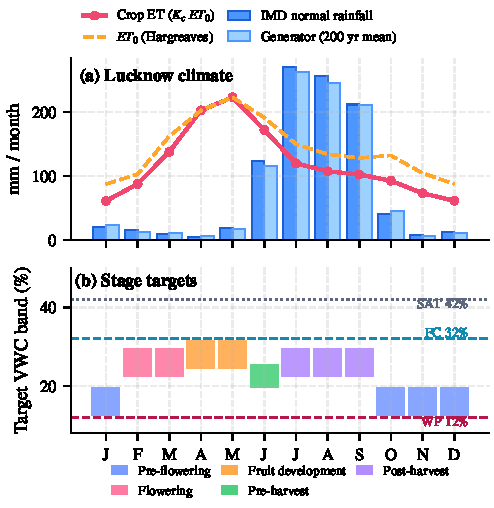
\includegraphics[width=\columnwidth]{fig3_climate_bands.pdf}
\caption{(a) IMD monthly rainfall normals for Lucknow versus the generator mean over 200 years, with Hargreaves $ET_0$ and crop evapotranspiration. (b) Stage-specific target bands relative to wilting point (WP), field capacity (FC) and saturation (SAT).}
\label{fig:climate}
\end{figure}

\subsection{DQN Formulation and Training}
\begin{itemize}
\item \textit{State (12 values):} scaled soil moisture, one-hot growth stage (5), maximum temperature, humidity, rain today, forecast rain, days since irrigation and $ET_0$.
\item \textit{Actions:} 0, 6, 12 or 20~mm of irrigation per day.
\item \textit{Reward:} $+1$ inside the band; outside it a penalty of 0.25 per percentage point on the dry side and 0.10 on the wet side; water cost 0.03 per mm; $-1$ for irrigating soil already above the band; $-0.5$ for irrigating when at least 8~mm of rain is forecast; and $-0.01$ per mm of drainage.
\item \textit{Network and training:} a 12--64--64--4 ReLU network implemented in NumPy, Double-DQN targets~\cite{vanhasselt2016}, Huber loss, Adam~\cite{kingma2015} (learning rate $10^{-3}$), batch 64, a 30\,000-transition replay buffer with 1000 warm-up transitions, target synchronisation every 400 updates, discount factor 0.97, and $\epsilon$-greedy exploration decayed linearly from 1.0 to 0.05 over the first 420 of 700 episodes. Each episode is one synthetic year (training seeds 1--700).
\end{itemize}

\subsection{Policies and Evaluation Protocol}
Five policies are compared: \textit{no irrigation}; a \textit{fixed schedule} of 12~mm every third day; a \textit{threshold rule} that irrigates toward the band centre (at most 20~mm) whenever soil moisture falls below the lower limit; the \textit{DQN} alone; and the \textit{agentic} configuration (DQN + guard) intended for deployment. Every policy is run on the same 30 weather years (seeds 10001--10030) that were never used in training. Paired differences are tested with the two-sided Wilcoxon signed-rank test. To isolate the guard, a stress test injects three probe faults for 60 days in the high-demand fruit-development period (days 91--150): a dead probe reporting 0\%, a reading frozen at its last value, and a dry drift of $-6$ percentage points.

\section{Implementation}

\subsection{Software Organisation}
The full system comprises the field firmware, the backend, the dashboard and the agent (Table~\ref{tab:repo}). The simulator, learning and guard modules used for every result in this paper are released as a self-contained reproducibility package with 20 unit tests covering the water balance, weather calibration, guard rules, sensor-health checks and the learner.

\begin{table}[!t]
\caption{Code Organisation of the Full System}
\label{tab:repo}
\centering
\footnotesize
\renewcommand{\arraystretch}{1.12}
\begin{tabular}{@{}>{\raggedright\arraybackslash}p{0.34\columnwidth}>{\raggedright\arraybackslash}p{0.58\columnwidth}@{}}
\toprule
\textbf{Path} & \textbf{Content} \\
\midrule
\texttt{mangoagent/} & config, weather, env (simulator), dqn, policies (baselines and guard), agent \\
\texttt{scripts/} & train\_dqn.py, evaluate.py, make\_figures.py \\
\texttt{tests/} & pytest unit tests \\
\texttt{results/} & weights, per-year results, traces, decision logs, statistics \\
\texttt{backend/} & FastAPI app, SQLite, MQTT bridge \\
\texttt{dashboard/} & Single-page web dashboard \\
\texttt{firmware/} & ESP32 Arduino sketch for the field node \\
\bottomrule
\end{tabular}
\end{table}

\subsection{Hardware}
The components of each field node are listed in Table~\ref{tab:hw}.

\begin{table}[!t]
\caption{Hardware List (Per Node)}
\label{tab:hw}
\centering
\footnotesize
\renewcommand{\arraystretch}{1.12}
\begin{tabular}{@{}>{\raggedright\arraybackslash}p{0.36\columnwidth}>{\raggedright\arraybackslash}p{0.56\columnwidth}@{}}
\toprule
\textbf{Item} & \textbf{Notes} \\
\midrule
ESP32 development board & Use ADC1 pins; ADC2 is unavailable while Wi-Fi is active \\
Capacitive soil-moisture sensor v1.2 & Two-point calibration in the local soil is essential~\cite{placidi2020} \\
DHT22 & Air temperature and humidity \\
Relay module, 12~V solenoid valve & Fail-safe: valve closed at start-up; firmware caps any command at 240~min \\
Li-ion cell, 1:2 divider, solar panel & Battery voltage reported; alert below 3.4~V \\
Weatherproof enclosure & Sealed cable glands; probe electronics above ground \\
\bottomrule
\end{tabular}
\end{table}

\section{Results}

\subsection{Training}
Fig.~\ref{fig:train} shows the learning curve. The mean return rose from $-615$ over the first ten episodes to $146\pm51$ over the last hundred, and stabilised once exploration reached its floor at episode 420. Training took about two minutes on two CPU cores.

\begin{figure}[!t]
\centering
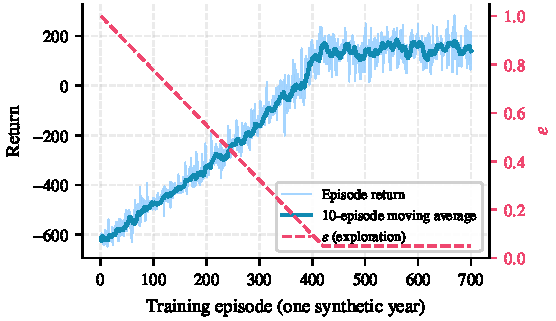
\includegraphics[width=\columnwidth]{fig4_training_curve.pdf}
\caption{Double-DQN training curve with the exploration rate $\epsilon$.}
\label{fig:train}
\end{figure}

\subsection{Policy Comparison}
Table~\ref{tab:results} and Fig.~\ref{fig:policies} summarise the 30 test years. The agentic policy kept the root zone in the band on 72.2\% of days, 8.8 percentage points more than the threshold rule ($p=1.7\times10^{-6}$), and cut days below the band from 9.8\% to 1.0\% ($p=1.7\times10^{-6}$). It used 748~mm per year, 7~mm (0.9\%) more than the threshold rule ($p=0.007$), with no significant difference in drainage ($p=0.56$). The fixed schedule applied 1464~mm, about twice the water of the adaptive policies, yet was in band on only 9.6\% of days and lost 1035~mm to drainage. Without irrigation the soil was below the band on 42.3\% of days and near wilting on 105 days per year outside the pre-flowering phase; every irrigated policy reduced this to essentially zero.

\begin{table*}[!t]
\caption{Simulated Yearly Performance on 30 Unseen Weather Years (Mean $\pm$ SD)}
\label{tab:results}
\centering
\renewcommand{\arraystretch}{1.12}
\begin{tabular}{@{}lcccccc@{}}
\toprule
\textbf{Policy} & \textbf{In band (\%)} & \textbf{Below band (\%)} & \textbf{Above band (\%)} & \textbf{Water (mm/yr)} & \textbf{Drainage (mm/yr)} & \textbf{Events/yr} \\
\midrule
No irrigation & 33.9 $\pm$ 5.7 & 42.3 $\pm$ 4.6 & 23.8 $\pm$ 6.8 & 0 & 364 $\pm$ 239 & 0 \\
Fixed schedule & 9.6 $\pm$ 3.2 & 16.3 $\pm$ 1.8 & 74.1 $\pm$ 3.9 & 1464 $\pm$ 0 & 1035 $\pm$ 280 & 122 \\
Threshold rule & 63.4 $\pm$ 5.4 & 9.8 $\pm$ 0.8 & 26.8 $\pm$ 5.8 & 741 $\pm$ 61 & 415 $\pm$ 239 & 37.2 \\
DQN alone & 72.3 $\pm$ 5.9 & 0.6 $\pm$ 0.4 & 27.1 $\pm$ 6.0 & 751 $\pm$ 65 & 416 $\pm$ 239 & 98.2 \\
Agentic (DQN + guard) & \textbf{72.2 $\pm$ 5.7} & \textbf{1.0 $\pm$ 0.9} & 26.9 $\pm$ 6.0 & 748 $\pm$ 67 & 413 $\pm$ 237 & 94.2 \\
\bottomrule
\end{tabular}
\end{table*}

\begin{figure*}[!t]
\centering
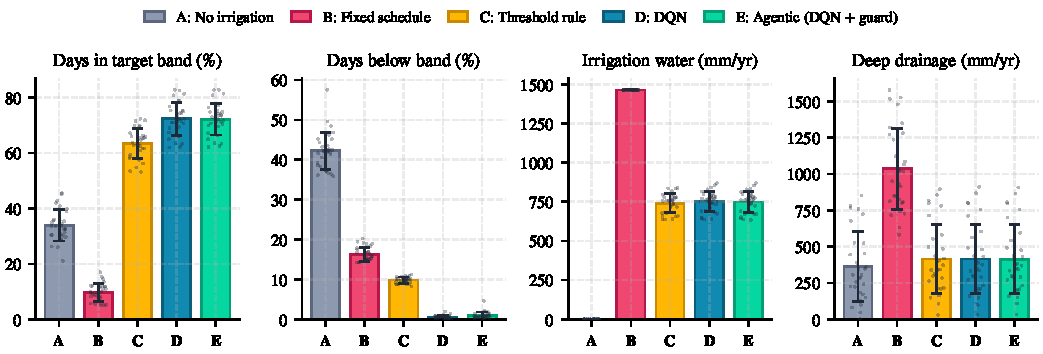
\includegraphics[width=\textwidth]{fig5_policy_comparison.pdf}
\caption{Policy comparison over 30 unseen weather years. Bars show means, error bars one standard deviation, and dots individual years.}
\label{fig:policies}
\end{figure*}

\begin{figure*}[!t]
\centering
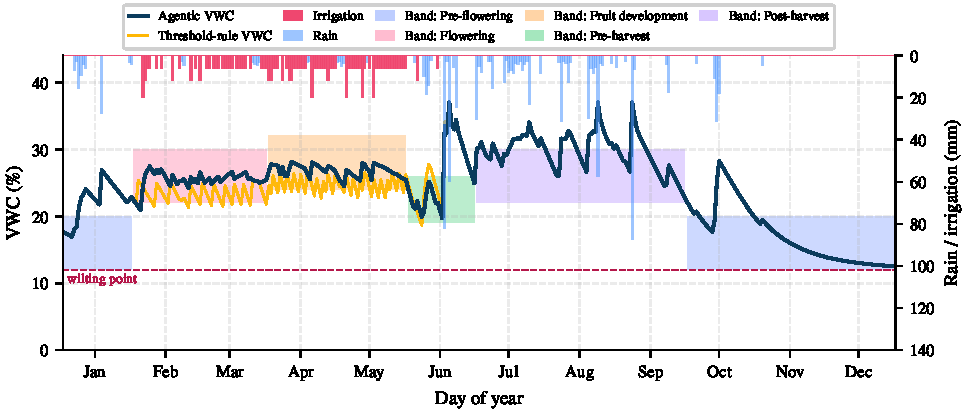
\includegraphics[width=\textwidth]{fig6_year_trace.pdf}
\caption{One test year (seed 10030). Shaded areas are the stage bands. The agentic policy irrigates in small, frequent events from February to May and applies no water in the pre-flowering phase; the threshold rule oscillates near the lower limit. From the monsoon onset both policies stop irrigating, so their traces coincide.}
\label{fig:year}
\end{figure*}

Fig.~\ref{fig:year} illustrates the difference. The threshold rule waits until the soil crosses the lower limit and then refills it, so it spends part of every cycle below the band. The learned policy irrigates earlier and in smaller amounts (94 events per year against 37), keeping moisture near the middle of the band at almost the same total water. All irrigated policies spend about 27\% of days above the band, almost entirely during the monsoon when rainfall exceeds crop demand.

\subsection{Contribution of the Safety Guard}
Under normal operation the guard altered 7.8$\pm$3.7 proposals per year (range 1--16): 75\% because rain was falling or forecast, 24\% because the seven-day budget was reached, and the rest for the stage, band or emergency rules. This saved 3~mm of water and 3~mm of drainage per year relative to the DQN alone ($p=0.009$), at the cost of 0.4 percentage points more days below the band ($p=0.0015$), because some forecast rain did not arrive. Table~\ref{tab:faults} and Fig.~\ref{fig:faults} show why the guard is nevertheless essential. With a dead probe reporting 0\%, the DQN alone applied the maximum 20~mm every day, 1200~mm in 60 days, of which 759~mm drained; the guard applied none and raised an alert on every faulty day. A frozen reading was detected after three days, limiting irrigation to 16~mm instead of 577~mm. A dry drift of $-6$ points, however, looks like a plausible reading and cannot be detected by the guard; it reduced over-irrigation only through its rain and budget rules (481~mm instead of 564~mm).

\begin{table}[!t]
\caption{Sensor-Fault Stress Test (Days 91--150, Mean of 30 Years)}
\label{tab:faults}
\centering
\footnotesize
\renewcommand{\arraystretch}{1.12}
\begin{tabular}{@{}llcccc@{}}
\toprule
\textbf{Fault} & \textbf{Policy} & \textbf{Water} & \textbf{Drain.} & \textbf{In band} & \textbf{Alert} \\
 & & \textbf{(mm)} & \textbf{(mm)} & \textbf{(\%)} & \textbf{days} \\
\midrule
\multirow{2}{*}{Dead probe (0\%)} & DQN & 1200 & 759 & 2.4 & -- \\
 & Agentic & 0 & 0 & 3.0 & 60 \\
\multirow{2}{*}{Frozen reading} & DQN & 577 & 186 & 38.6 & -- \\
 & Agentic & 16 & 0 & 7.1 & 58 \\
\multirow{2}{*}{Dry drift ($-6$ pp)} & DQN & 564 & 136 & 27.7 & -- \\
 & Agentic & 481 & 56 & 56.6 & 0 \\
\bottomrule
\end{tabular}
\end{table}

\begin{figure*}[!t]
\centering
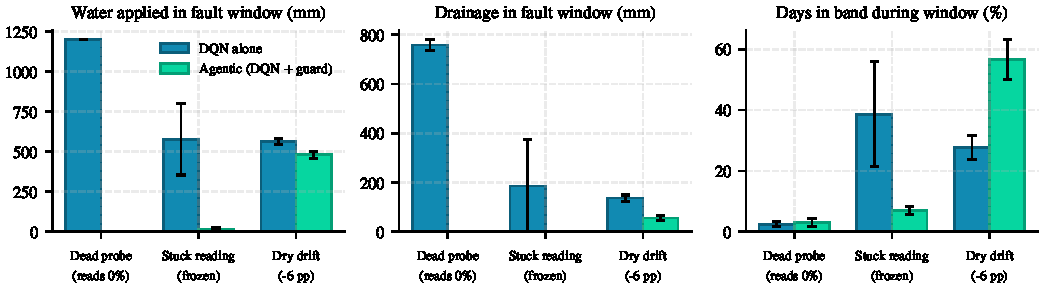
\includegraphics[width=\textwidth]{fig7_fault_test.pdf}
\caption{Sensor-fault stress test over a 60-day window in the fruit-development stage. The guard stops erroneous irrigation for detectable faults (dead and frozen probe) but not for a plausible drift.}
\label{fig:faults}
\end{figure*}

\section{Discussion}
\begin{itemize}
\item \textit{Adaptive control outperforms the calendar.} The fixed schedule ignores rain and growth stage; its 1035~mm of drainage is the clearest evidence of waste.
\item \textit{The learned policy reduces stress at almost no water cost.} Relative to the threshold rule, the agentic policy adds 8.8 days in every hundred inside the band and nearly eliminates days below it for 0.9\% more water. Its value in practice depends on the cost of water and of a day of stress, neither of which is measured here.
\item \textit{The guard trades a little performance for robustness.} In fault-free simulation the guard is slightly conservative, but it is the only component that prevents a single dead probe from flooding the orchard. When it blocks irrigation because of a fault, the farmer must act on the alert; a fallback schedule would avoid the resulting dry period and is planned.
\item \textit{Days above the band are caused by rain.} About 27\% of days lie above the band for every irrigated policy, mainly in the monsoon, when no valve can remove water. Drainage, mulching or raised beds address this, not a cleverer controller.
\item \textit{Year-to-year variation is large.} Standard deviations of 5--6 percentage points mean that a one-season field comparison could mislead; trials should span several seasons.
\end{itemize}

\section{Limitations and Validation Plan}
\label{sec:limits}
\begin{itemize}
\item Soil constants, band limits and crop coefficients are assumed. Field capacity, wilting point and the bands must be calibrated through soil tests with an agronomist and checked against a tensiometer or neutron-probe reference.
\item Weather is generated from climatological normals with a single soil layer. The policy should be retrained and tested on recorded station weather from the site, and a multi-layer root-zone model considered for deep-rooted trees.
\item The learner has no model of yield or fruit quality. A field trial should compare agent-managed and grower-managed blocks, recording yield, fruit size and water use.
\item Capacitive probes drift with temperature and salinity, and the guard cannot detect a plausible drift; seasonal recalibration and cross-checks with manual readings are required.
\item Before deployment the system must be secured (API key, MQTT authentication and TLS, HTTPS), and manual override must remain available; the firmware's local timer closes the valve if the network fails.
\end{itemize}

\section{Conclusion}
This paper presented an agentic AI and IoT irrigation system for mango orchards that combines ESP32 field nodes, an MQTT/HTTP backend, a Double-DQN planner, a deterministic safety guard and a farmer-facing dashboard. In a simulator calibrated to IMD climate normals for Lucknow, the agentic policy kept the root zone inside the stage-specific band on 72.2\% of days over 30 unseen years, compared with 63.4\% for a threshold rule, and reduced days below the band from 9.8\% to 1.0\% for 0.9\% more water. The guard prevented a dead sensor from triggering 1200~mm of erroneous irrigation in 60 days. These results are conditional on assumed soil and crop parameters; future work will calibrate the model with site data, add a fault-tolerant fallback schedule and validate the system in a multi-season field trial against grower practice.

\section*{Data and Code Availability}
The simulator, training and evaluation scripts, per-year results, decision logs and figure scripts are provided with this paper; running \texttt{scripts/train\_dqn.py}, \texttt{scripts/evaluate.py} and \texttt{scripts/make\_figures.py} reproduces every number and figure.

\section*{Acknowledgment}
An AI writing and coding assistant was used to help draft text, implement the simulation code and prepare figures; the author reviewed, verified and takes full responsibility for all content, data and references.

\begin{thebibliography}{00}
\bibitem{ntdaf} Y. Diczbalis, C. Wicks, and G. Owens, ``Mango irrigation management guidelines,'' Agnote D14, Dept. of Primary Industry, Fisheries and Mines, Northern Territory Government, Darwin, Australia, 2006. [Online]. Available: \url{https://daf.nt.gov.au/__data/assets/pdf_file/0004/232969/587.pdf}
\bibitem{wfp} Growcom, ``Water for Profit benchmark: Irrigating mangoes in north Queensland,'' Growcom, Queensland, Australia. [Online]. Available: \url{https://www.industry.mangoes.net.au/cmsb/uploads/wfp-benchmark-irrigating-mangoes-in-north-queensland.pdf}
\bibitem{garcia2020} L. Garc\'{\i}a \textit{et al.}, ``IoT-based smart irrigation systems: An overview on the recent trends on sensors and IoT systems for irrigation in precision agriculture,'' \textit{Sensors}, vol. 20, no. 4, Art. no. 1042, 2020, doi: 10.3390/s20041042.
\bibitem{goap2018} A. Goap, D. Sharma, A. K. Shukla, and C. Rama Krishna, ``An IoT based smart irrigation management system using machine learning and open source technologies,'' \textit{Comput. Electron. Agric.}, vol. 155, pp. 41--49, 2018.
\bibitem{chen2021} M. Chen \textit{et al.}, ``A reinforcement learning approach to irrigation decision-making for rice using weather forecasts,'' \textit{Agric. Water Manag.}, vol. 250, Art. no. 106838, 2021, doi: 10.1016/j.agwat.2021.106838.
\bibitem{alibabaei2022} K. Alibabaei \textit{et al.}, ``Comparison of on-policy deep reinforcement learning A2C with off-policy DQN in irrigation optimization: A case study at a site in Portugal,'' \textit{Computers}, vol. 11, no. 7, Art. no. 104, 2022, doi: 10.3390/computers11070104.
\bibitem{ding2022} X. Ding and W. Du, ``DRLIC: Deep reinforcement learning for irrigation control,'' in \textit{Proc. 21st ACM/IEEE Int. Conf. Inf. Process. Sensor Netw. (IPSN)}, Milan, Italy, 2022.
\bibitem{mnih2015} V. Mnih \textit{et al.}, ``Human-level control through deep reinforcement learning,'' \textit{Nature}, vol. 518, no. 7540, pp. 529--533, 2015, doi: 10.1038/nature14236.
\bibitem{yao2023} S. Yao \textit{et al.}, ``ReAct: Synergizing reasoning and acting in language models,'' in \textit{Proc. 11th Int. Conf. Learn. Represent. (ICLR)}, 2023.
\bibitem{samant2017} D. Samant, S. Mandal, V. Nath, and R. M. Kurian, ``Effect of deficit drip irrigation and mulching on mango hybrid `Amrapali','' \textit{J. Indian Soc. Coastal Agric. Res.}, vol. 35, no. 2, 2017.
\bibitem{hahn2022} F. Hahn and J. A. Garcia, ``Mango stem response under different irrigation regimes,'' \textit{Int. J. Fruit Sci.}, vol. 22, no. 1, 2022, doi: 10.1080/15538362.2021.1970080.
\bibitem{spreer2009} W. Spreer, S. Ongprasert, M. Hegele, J. N. W\"{u}nsche, and J. M\"{u}ller, ``Yield and fruit development in mango (\textit{Mangifera indica} L. cv. Chok Anan) under different irrigation regimes,'' \textit{Agric. Water Manag.}, vol. 96, no. 4, pp. 574--584, 2009.
\bibitem{placidi2020} P. Placidi \textit{et al.}, ``Characterization of low-cost capacitive soil moisture sensors for IoT networks,'' \textit{Sensors}, vol. 20, no. 12, Art. no. 3585, 2020, doi: 10.3390/s20123585.
\bibitem{vanhasselt2016} H. van Hasselt, A. Guez, and D. Silver, ``Deep reinforcement learning with double Q-learning,'' in \textit{Proc. AAAI Conf. Artif. Intell.}, vol. 30, no. 1, 2016, pp. 2094--2100.
\bibitem{imd} India Meteorological Department, ``Climatology of Lucknow,'' Meteorological Centre, Lucknow. [Online]. Available: \url{https://mausam.imd.gov.in/lucknow/mcdata/climatology_lucknow.pdf}
\bibitem{allen1998} R. G. Allen, L. S. Pereira, D. Raes, and M. Smith, ``Crop evapotranspiration: Guidelines for computing crop water requirements,'' FAO Irrigation and Drainage Paper 56, FAO, Rome, Italy, 1998.
\bibitem{hargreaves2003} G. H. Hargreaves and R. G. Allen, ``History and evaluation of Hargreaves evapotranspiration equation,'' \textit{J. Irrig. Drain. Eng.}, vol. 129, no. 1, pp. 53--63, 2003.
\bibitem{kingma2015} D. P. Kingma and J. Ba, ``Adam: A method for stochastic optimization,'' in \textit{Proc. 3rd Int. Conf. Learn. Represent. (ICLR)}, 2015.
\end{thebibliography}

\end{document}
